%!TEX root = ../paper.tex
%!TEX encoding = UTF-8 Unicode

\section{Evaluation}
\label{sec:evaluation}

In order to evaluate our approach, we integrated a Shuttle prototype with AppScale and Voldemort. AppScale \cite{Appscale} is an open-source version of Google App Engine. Voldemort \cite{Kreps} is an open source implementation of Dynamo \cite{Decandia2007}, developed and in use by LinkedIn. Shuttle’s prototype has been developed in Java (1400 lines of code for the proxy, 1800 for the manager, 300 for the interceptor, 900 for the replay instances and 1800 for the database proxy).


\subsection{Application Example: Ask}
\label{sec:evaluation:app}

We developed a \acf{QA} web application for \ac{PaaS} inspired on Stack Exchange \footnote{http://stackexchange.com} (1700 lines of code) to evaluate Shuttle. The application represents a generic web application that accepts requests and stores the persistent state in the Voldemort database. Its implementation is independent of Shuttle, i.e., Shuttle does not require the application to be modified. 

The application semantics implies the following dependencies: a) questions are independent; b) new answers depend from previous answers and votes to the same question; c) new comments depend from the commented answer; d) news vote depend from the voted answer. We selected subsets of a dump of the Stack Exchange database \footnote{Available in: https://archive.org/details/stackexchange} to simulate real-world requests. 

\subsection{Accuracy}
\label{sec:evaluation:accuracy}

We evaluate Shuttle's ability to correctly recovery applications in different scenarios. We consider three classes of intrusion scenarios: malicious requests, software vulnerabilities and external channels (e.g. SSH connections). The selected data subset contains 100 000 requests originally performed from 31 July until 12 Sep.~2008: 6992 questions, 28993 answers, 2220 comments, 61795 votes and 3062 tags. Requests were sorted per date, establishing 92 939 dependencies.

At intrusion moment, Sep.~2nd, the database contains 4338 questions, 18286 answers, 422 comments and 38334 votes (61380 requests). The attack is detected in Sep.~12th, assuming a pessimistic delay of 10 days. During this period, the application retrieved 38 620 requests. Table \ref{tab:accuracy} represents the summary of the accuracy tests. It contains the number of data items tampered by the intrusion (\emph{\#intrusion}) and the number of user requests that read data items written by  tainted requests or malicious requests (without considering the intrusion requests). Recovery using \textit{full replay} requires to replay every request from the latest snapshot before the intrusion instant until the detection instant: in this example at least 38 620 requests (\emph{\#replayed (fr)}). Selective replay only re-executes tainted requests, unless some data item versions need to be recreated. On the worst case, the system does not contain any snapshot and every data read by the tainted requests shall be recreated (\emph{\#replayed (sr)}). 

\begin{table}
\footnotesize
\begin{tabular}{l|rrrr}
    & \#intrusion & \#tainted & \#replayed (sr)     & \#replayed (fr) \\ \hline
1a       & 110          & 0          & $[0, 605]$   & $> 38 620$  \\
1b       & 58           & 14         & $[0, 379]$   & $> 38 620$  \\
1c       & 48           & 52         & $[0, 253]$   & $> 38 620$  \\
2a       & 4 338        & 0          &  -           & $> 38 620$  \\
2b       & 18 286       & 1 278      &  -           & $> 38 620$  \\
3        & 2 000        & -          &  -           & $> 38 620$  \\
\end{tabular}
  \caption{Number of requests replayed during the recovery process}
  \label{tab:accuracy}
  \vspace{-5mm}
\end{table}


%Scenario A: tainted request
\textbf{Malicious Requests.} 
 In the first class of scenarios, we consider three  cases in which an attacker has stolen an user credential, then: a) deleted every question created by the user; b) deleted every user answer; or c) modified every user answer.

\textit{1a)} The attacker deletes the user's 4 questions, performing 4 delete requests that remove 106 associated comments and answers. The tenant identifies the malicious requests through the user session and selects a snapshot previous to the intrusion instant. Users cannot access deleted questions, so no request is tainted. If Shuttle has a snapshot containing the deleted questions, then \textit{selective replay} does not need to replay any request and merges the deleted questions on the current system state. If the latest snapshot is previous to the creation of the 4 questions, then \textit{selective replay} replays 605 requests to recreate the deleted questions, their answers and votes. The result is merged with the current branch, rebuilding the deleted questions. 

\textit{1b)} Deleting the user's 48 answers implies that 58 data items are deleted and 14 answers and comments are tainted as they execute after the intrusion instant answering and voting without knowing some answers. If a snapshot containing the user answers exists, then the \textit{selective replay} approach replays only 14 tainted answers and comments. Otherwise, it replays 379 requests: the total number of requests to recreate the tainted questions and then merge the result.


\textit{1c)} 48 data items are modified while 52 requests are tainted because the users replays, votes and comments the modified questions after the intrusion instant. For recovery, the 52 tainted requests shall be replayed. If Shuttle does not have a snapshot containing the questions, then 253 requests have to be replayed to recreate them. 

\textbf{Software vulnerability.}
On the second class, we evaluate intrusion scenarios where software flaws allow attackers to modify the database without authorization. For instance, a code version added a flaw that allows \emph{SQL-Injection}. We consider two independent scenarios where the attacker: a) deleted every question; b) deleted every answer.

In \textit{2a)}, the deleting of every question removes 4 338 data items. In \textit{2b)}, the questions are preserved but 1 278 answers, votes and comments are tainted as the user did not see the deleted answers.

Instead of identifying the requests that explored the vulnerability, the tenant patches the code to remove the application vulnerability. Tenants use the instance rejuvenation mechanism to shutdown current application containers and deploy new application version. After, they use the \textit{full replay} to repeat all requests since the beginning of usage of the software version with the flaw. Requests that explored the vulnerability fail to execute and a consistent application state is recovered.\\



\textbf{External channel.}
On the third class, we consider a case where the proxy does not log the attacker actions. In this case, an attacker used a SSH account created by exploring the shellsock, which is a bash vulnerability. The attacker stolen the database credentials and modified at least 2000 data items. Since these database operations are not logged, the dependencies are not established and the number of tainted requests is unknown. However, even without logging the malicious actions, Shuttle recovers the application by loading a database snapshot previous to the estimated intrusion instant (Sep.~2nd) and performing \textit{full replay}. The attack effects are removed because Shuttle loads a database snapshot instead of undoing every operation. As the malicious actions were not logged, they are not replayed and Shuttle recovers the application consistency.\\


The number of requests to replay is defined by the snapshot instant: on \textit{full replay} Shuttle replays all requests performed after the intrusion instant, while on \textit{selective replay} Shuttle replays the requests necessary to read the values of the entries before the intrusion and the tainted requests. While  \textit{selective replay} seems to have a big advantage comparing with  \textit{full replay}, which performs, in these scenarios, at least 38 620 requests, most real applications have more dependencies thus the number of tainted requests is bigger. For instance, if the order between questions with the same tag is considered as a dependency,  the number of dependencies rises from 92 939 to 109 118 and the number of independent clusters decreases from 6992 to 56. We plan to further analyze the dependencies established by different applications. 



\subsection{Performance}
\label{sec:evaluation:performance}

We evaluate Shuttle's performance considering the throughput of the application, the size of the logs and the recovery time. We also estimate the cost of deployment of Shuttle on a public cloud provider \acf{AWS}. We run 6 \ac{AWS} \textit{c3.xlarge} instances (14 ECUs, 4 vCPUs, 2.8 GHz, Intel Xeon E5-2680v2, 7.5 GB of memory, 2 x 40 GB Storage Capacity) connected by gigabit ethernet (780Mbps measured with \emph{iperf}, 0.176ms round-trip time measured with \emph{ping}). We use one client, one instance with Shuttle proxy and a load balancer (HAProxy), three WildFly (formerly known as JBoss) application servers and one Voldemort database. We consider a large data sample from the data of Stack Exchange with 50 000 requests (1432 questions, 3399 answers, 8335 comments, 36834 votes, 950 000 question views). We do not consider a particular scenario or replay scheme (full/selective), but define instead the number of requests recovered per experiment.

\textbf{Performance overhead.}
We evaluate the overhead of Shuttle by measuring the throughput of the \textit{Ask} application with and without Shuttle (Table \ref{tab:throughput}). We considered two workloads: (A) has 50\% reads, 50\% write and (B) has 95\% reads, 5\% write. Write operations insert questions, answers, comments and votes of the data sample, while the read operations access the latest inserted questions. Table \ref{tab:throughput} shows that Shuttle imposes an overhead of 13-20\%, which seems reasonable considering the benefits of having it. We believe the main cause of overhead is the current proxy, which is not very optimized. The current version written in Java performs considerably better than a previous version in Python, but we expect to be able to do much better by rewriting it in C.\\

\begin{table}
\footnotesize
\begin{tabular}{l|rr}
                       &  Workload A                    & Workload B  \\ \hline
Shuttle                &  6325 ops/sec [5.78 ms]        &  15346 ops/sec [3.62 ms]  \\
No Shuttle             &  7148 ops/sec [5.07 ms]        &  17821 ops/sec [3.01 ms]  \\
overhead               &  13\% [14\%]                    & 16\% [20\%] \\
\end{tabular}
\caption{Shuttle overhead in terms of application throughput (ops/sec) and response latency (ms)}
\label{tab:throughput}
\vspace{-3mm}
\end{table}

%\hl{estes resultados são estranhos, são tão bons quando comparados com os outros.}
%database overhead
In order to measure Shuttle's overhead on the database accesses, we used the \acf{YCSB} framework \cite{ycsb}. We considered two workloads: (A) has 50\% reads, 50\% updates and (B) has 95\% reads, 5\% updates. Operations access 1KB records following a Zipfian distribution (Figure \ref{fig:database_overhead}). Results show Shuttle has small impact on the latency of database accesses. 

\begin{figure}[tbh]
\vspace{-6mm}
\hspace*{-0.5cm}
  \LARGE
  \mbox{
      \subfloat[][Workload A - update \label{fig:database:a:update}]{
      \hspace{-0.5cm}
        \resizebox{4.5cm}{!}{% GNUPLOT: LaTeX picture with Postscript
\begingroup
  \makeatletter
  \providecommand\color[2][]{%
    \GenericError{(gnuplot) \space\space\space\@spaces}{%
      Package color not loaded in conjunction with
      terminal option `colourtext'%
    }{See the gnuplot documentation for explanation.%
    }{Either use 'blacktext' in gnuplot or load the package
      color.sty in LaTeX.}%
    \renewcommand\color[2][]{}%
  }%
  \providecommand\includegraphics[2][]{%
    \GenericError{(gnuplot) \space\space\space\@spaces}{%
      Package graphicx or graphics not loaded%
    }{See the gnuplot documentation for explanation.%
    }{The gnuplot epslatex terminal needs graphicx.sty or graphics.sty.}%
    \renewcommand\includegraphics[2][]{}%
  }%
  \providecommand\rotatebox[2]{#2}%
  \@ifundefined{ifGPcolor}{%
    \newif\ifGPcolor
    \GPcolorfalse
  }{}%
  \@ifundefined{ifGPblacktext}{%
    \newif\ifGPblacktext
    \GPblacktexttrue
  }{}%
  % define a \g@addto@macro without @ in the name:
  \let\gplgaddtomacro\g@addto@macro
  % define empty templates for all commands taking text:
  \gdef\gplbacktext{}%
  \gdef\gplfronttext{}%
  \makeatother
  \ifGPblacktext
    % no textcolor at all
    \def\colorrgb#1{}%
    \def\colorgray#1{}%
  \else
    % gray or color?
    \ifGPcolor
      \def\colorrgb#1{\color[rgb]{#1}}%
      \def\colorgray#1{\color[gray]{#1}}%
      \expandafter\def\csname LTw\endcsname{\color{white}}%
      \expandafter\def\csname LTb\endcsname{\color{black}}%
      \expandafter\def\csname LTa\endcsname{\color{black}}%
      \expandafter\def\csname LT0\endcsname{\color[rgb]{1,0,0}}%
      \expandafter\def\csname LT1\endcsname{\color[rgb]{0,1,0}}%
      \expandafter\def\csname LT2\endcsname{\color[rgb]{0,0,1}}%
      \expandafter\def\csname LT3\endcsname{\color[rgb]{1,0,1}}%
      \expandafter\def\csname LT4\endcsname{\color[rgb]{0,1,1}}%
      \expandafter\def\csname LT5\endcsname{\color[rgb]{1,1,0}}%
      \expandafter\def\csname LT6\endcsname{\color[rgb]{0,0,0}}%
      \expandafter\def\csname LT7\endcsname{\color[rgb]{1,0.3,0}}%
      \expandafter\def\csname LT8\endcsname{\color[rgb]{0.5,0.5,0.5}}%
    \else
      % gray
      \def\colorrgb#1{\color{black}}%
      \def\colorgray#1{\color[gray]{#1}}%
      \expandafter\def\csname LTw\endcsname{\color{white}}%
      \expandafter\def\csname LTb\endcsname{\color{black}}%
      \expandafter\def\csname LTa\endcsname{\color{black}}%
      \expandafter\def\csname LT0\endcsname{\color{black}}%
      \expandafter\def\csname LT1\endcsname{\color{black}}%
      \expandafter\def\csname LT2\endcsname{\color{black}}%
      \expandafter\def\csname LT3\endcsname{\color{black}}%
      \expandafter\def\csname LT4\endcsname{\color{black}}%
      \expandafter\def\csname LT5\endcsname{\color{black}}%
      \expandafter\def\csname LT6\endcsname{\color{black}}%
      \expandafter\def\csname LT7\endcsname{\color{black}}%
      \expandafter\def\csname LT8\endcsname{\color{black}}%
    \fi
  \fi
  \setlength{\unitlength}{0.0500bp}%
  \begin{picture}(7200.00,5040.00)%
    \gplgaddtomacro\gplbacktext{%
      \csname LTb\endcsname%
      \put(1078,704){\makebox(0,0)[r]{\strut{} 0}}%
      \put(1078,1629){\makebox(0,0)[r]{\strut{} 500}}%
      \put(1078,2554){\makebox(0,0)[r]{\strut{} 1000}}%
      \put(1078,3480){\makebox(0,0)[r]{\strut{} 1500}}%
      \put(1078,4405){\makebox(0,0)[r]{\strut{} 2000}}%
      \put(1210,484){\makebox(0,0){\strut{} 5}}%
      \put(2009,484){\makebox(0,0){\strut{} 10}}%
      \put(2808,484){\makebox(0,0){\strut{} 15}}%
      \put(3607,484){\makebox(0,0){\strut{} 20}}%
      \put(4406,484){\makebox(0,0){\strut{} 25}}%
      \put(5205,484){\makebox(0,0){\strut{} 30}}%
      \put(6004,484){\makebox(0,0){\strut{} 35}}%
      \put(6803,484){\makebox(0,0){\strut{} 40}}%
      \put(176,2739){\rotatebox{-270}{\makebox(0,0){\strut{}Update latency (us)}}}%
      \put(4006,154){\makebox(0,0){\strut{}Throughput (thousand ops/sec)}}%
    }%
    \gplgaddtomacro\gplfronttext{%
      \csname LTb\endcsname%
      \put(5816,1416){\makebox(0,0)[r]{\strut{}Shuttle}}%
      \csname LTb\endcsname%
      \put(5816,1042){\makebox(0,0)[r]{\strut{}No Shuttle}}%
    }%
    \gplbacktext
    \put(0,0){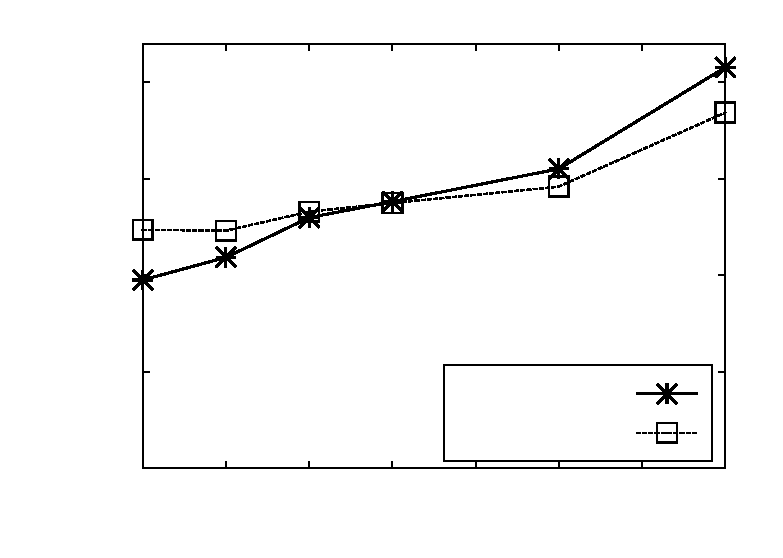
\includegraphics{graphs/database/a_update}}%
    \gplfronttext
  \end{picture}%
\endgroup
}
      }
      \subfloat[][Workload B - read \label{fig:database:b:read}]{
      \hspace{-0.7cm}
        \resizebox{4.5cm}{!}{% GNUPLOT: LaTeX picture with Postscript
\begingroup
  \makeatletter
  \providecommand\color[2][]{%
    \GenericError{(gnuplot) \space\space\space\@spaces}{%
      Package color not loaded in conjunction with
      terminal option `colourtext'%
    }{See the gnuplot documentation for explanation.%
    }{Either use 'blacktext' in gnuplot or load the package
      color.sty in LaTeX.}%
    \renewcommand\color[2][]{}%
  }%
  \providecommand\includegraphics[2][]{%
    \GenericError{(gnuplot) \space\space\space\@spaces}{%
      Package graphicx or graphics not loaded%
    }{See the gnuplot documentation for explanation.%
    }{The gnuplot epslatex terminal needs graphicx.sty or graphics.sty.}%
    \renewcommand\includegraphics[2][]{}%
  }%
  \providecommand\rotatebox[2]{#2}%
  \@ifundefined{ifGPcolor}{%
    \newif\ifGPcolor
    \GPcolorfalse
  }{}%
  \@ifundefined{ifGPblacktext}{%
    \newif\ifGPblacktext
    \GPblacktexttrue
  }{}%
  % define a \g@addto@macro without @ in the name:
  \let\gplgaddtomacro\g@addto@macro
  % define empty templates for all commands taking text:
  \gdef\gplbacktext{}%
  \gdef\gplfronttext{}%
  \makeatother
  \ifGPblacktext
    % no textcolor at all
    \def\colorrgb#1{}%
    \def\colorgray#1{}%
  \else
    % gray or color?
    \ifGPcolor
      \def\colorrgb#1{\color[rgb]{#1}}%
      \def\colorgray#1{\color[gray]{#1}}%
      \expandafter\def\csname LTw\endcsname{\color{white}}%
      \expandafter\def\csname LTb\endcsname{\color{black}}%
      \expandafter\def\csname LTa\endcsname{\color{black}}%
      \expandafter\def\csname LT0\endcsname{\color[rgb]{1,0,0}}%
      \expandafter\def\csname LT1\endcsname{\color[rgb]{0,1,0}}%
      \expandafter\def\csname LT2\endcsname{\color[rgb]{0,0,1}}%
      \expandafter\def\csname LT3\endcsname{\color[rgb]{1,0,1}}%
      \expandafter\def\csname LT4\endcsname{\color[rgb]{0,1,1}}%
      \expandafter\def\csname LT5\endcsname{\color[rgb]{1,1,0}}%
      \expandafter\def\csname LT6\endcsname{\color[rgb]{0,0,0}}%
      \expandafter\def\csname LT7\endcsname{\color[rgb]{1,0.3,0}}%
      \expandafter\def\csname LT8\endcsname{\color[rgb]{0.5,0.5,0.5}}%
    \else
      % gray
      \def\colorrgb#1{\color{black}}%
      \def\colorgray#1{\color[gray]{#1}}%
      \expandafter\def\csname LTw\endcsname{\color{white}}%
      \expandafter\def\csname LTb\endcsname{\color{black}}%
      \expandafter\def\csname LTa\endcsname{\color{black}}%
      \expandafter\def\csname LT0\endcsname{\color{black}}%
      \expandafter\def\csname LT1\endcsname{\color{black}}%
      \expandafter\def\csname LT2\endcsname{\color{black}}%
      \expandafter\def\csname LT3\endcsname{\color{black}}%
      \expandafter\def\csname LT4\endcsname{\color{black}}%
      \expandafter\def\csname LT5\endcsname{\color{black}}%
      \expandafter\def\csname LT6\endcsname{\color{black}}%
      \expandafter\def\csname LT7\endcsname{\color{black}}%
      \expandafter\def\csname LT8\endcsname{\color{black}}%
    \fi
  \fi
  \setlength{\unitlength}{0.0500bp}%
  \begin{picture}(7200.00,5040.00)%
    \gplgaddtomacro\gplbacktext{%
      \csname LTb\endcsname%
      \put(1078,704){\makebox(0,0)[r]{\strut{} 0}}%
      \put(1078,1629){\makebox(0,0)[r]{\strut{} 500}}%
      \put(1078,2554){\makebox(0,0)[r]{\strut{} 1000}}%
      \put(1078,3480){\makebox(0,0)[r]{\strut{} 1500}}%
      \put(1078,4405){\makebox(0,0)[r]{\strut{} 2000}}%
      \put(1210,484){\makebox(0,0){\strut{} 5}}%
      \put(2009,484){\makebox(0,0){\strut{} 10}}%
      \put(2808,484){\makebox(0,0){\strut{} 15}}%
      \put(3607,484){\makebox(0,0){\strut{} 20}}%
      \put(4406,484){\makebox(0,0){\strut{} 25}}%
      \put(5205,484){\makebox(0,0){\strut{} 30}}%
      \put(6004,484){\makebox(0,0){\strut{} 35}}%
      \put(6803,484){\makebox(0,0){\strut{} 40}}%
      \put(176,2739){\rotatebox{-270}{\makebox(0,0){\strut{}Read latency (us)}}}%
      \put(4006,154){\makebox(0,0){\strut{}Throughput (thousand ops/sec)}}%
    }%
    \gplgaddtomacro\gplfronttext{%
      \csname LTb\endcsname%
      \put(5816,1416){\makebox(0,0)[r]{\strut{}Shuttle}}%
      \csname LTb\endcsname%
      \put(5816,1042){\makebox(0,0)[r]{\strut{}No Shuttle}}%
    }%
    \gplbacktext
    \put(0,0){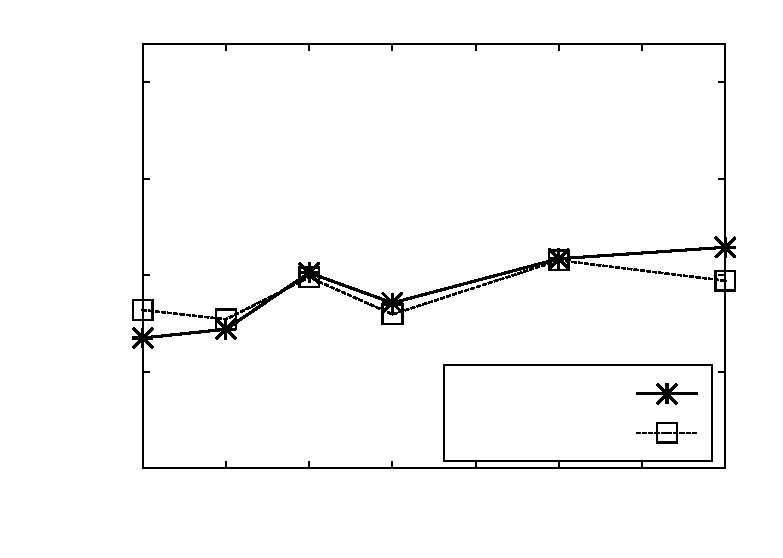
\includegraphics{graphs/database/b_read}}%
    \gplfronttext
  \end{picture}%
\endgroup
}
      }
  }
  \caption{Performance overhead on database}
  \vspace{-2mm}
  \label{fig:database_overhead}
\end{figure}


\textbf{Recovery.}
We measured the recovery time using Shuttle to replay the sample of 1 million requests. While serial replay (1 cluster) takes approximately half hour (1717s), recovery with clusters takes only 9 minutes (544s) (Figure \ref{fig:recovery_times}).

We measured the recovery period with different number of instances on clustered mode (Figure \ref{fig:scalability}). The figure shows that Shuttle is scalable, in the sense that adding more servers allow reducing the time of recovery (3 servers allowed recovery in half the time of 1, \~750 versus ~400 s). 

%Shuttle scalability: Recovery time considering the number of database and web-server instances and the number of acting users in parallel (runtime-recovery). On clustered mode, each cluster is replayed by one replay instance.
\begin{figure}[tbh]
\vspace{-5mm}
  \LARGE
  \mbox{
      \subfloat[][Recovery time \label{fig:recovery_times}]{
      \hspace{-0.5cm}
        \resizebox{4.5cm}{!}{% GNUPLOT: LaTeX picture with Postscript
\begingroup
  \makeatletter
  \providecommand\color[2][]{%
    \GenericError{(gnuplot) \space\space\space\@spaces}{%
      Package color not loaded in conjunction with
      terminal option `colourtext'%
    }{See the gnuplot documentation for explanation.%
    }{Either use 'blacktext' in gnuplot or load the package
      color.sty in LaTeX.}%
    \renewcommand\color[2][]{}%
  }%
  \providecommand\includegraphics[2][]{%
    \GenericError{(gnuplot) \space\space\space\@spaces}{%
      Package graphicx or graphics not loaded%
    }{See the gnuplot documentation for explanation.%
    }{The gnuplot epslatex terminal needs graphicx.sty or graphics.sty.}%
    \renewcommand\includegraphics[2][]{}%
  }%
  \providecommand\rotatebox[2]{#2}%
  \@ifundefined{ifGPcolor}{%
    \newif\ifGPcolor
    \GPcolorfalse
  }{}%
  \@ifundefined{ifGPblacktext}{%
    \newif\ifGPblacktext
    \GPblacktexttrue
  }{}%
  % define a \g@addto@macro without @ in the name:
  \let\gplgaddtomacro\g@addto@macro
  % define empty templates for all commands taking text:
  \gdef\gplbacktext{}%
  \gdef\gplfronttext{}%
  \makeatother
  \ifGPblacktext
    % no textcolor at all
    \def\colorrgb#1{}%
    \def\colorgray#1{}%
  \else
    % gray or color?
    \ifGPcolor
      \def\colorrgb#1{\color[rgb]{#1}}%
      \def\colorgray#1{\color[gray]{#1}}%
      \expandafter\def\csname LTw\endcsname{\color{white}}%
      \expandafter\def\csname LTb\endcsname{\color{black}}%
      \expandafter\def\csname LTa\endcsname{\color{black}}%
      \expandafter\def\csname LT0\endcsname{\color[rgb]{1,0,0}}%
      \expandafter\def\csname LT1\endcsname{\color[rgb]{0,1,0}}%
      \expandafter\def\csname LT2\endcsname{\color[rgb]{0,0,1}}%
      \expandafter\def\csname LT3\endcsname{\color[rgb]{1,0,1}}%
      \expandafter\def\csname LT4\endcsname{\color[rgb]{0,1,1}}%
      \expandafter\def\csname LT5\endcsname{\color[rgb]{1,1,0}}%
      \expandafter\def\csname LT6\endcsname{\color[rgb]{0,0,0}}%
      \expandafter\def\csname LT7\endcsname{\color[rgb]{1,0.3,0}}%
      \expandafter\def\csname LT8\endcsname{\color[rgb]{0.5,0.5,0.5}}%
    \else
      % gray
      \def\colorrgb#1{\color{black}}%
      \def\colorgray#1{\color[gray]{#1}}%
      \expandafter\def\csname LTw\endcsname{\color{white}}%
      \expandafter\def\csname LTb\endcsname{\color{black}}%
      \expandafter\def\csname LTa\endcsname{\color{black}}%
      \expandafter\def\csname LT0\endcsname{\color{black}}%
      \expandafter\def\csname LT1\endcsname{\color{black}}%
      \expandafter\def\csname LT2\endcsname{\color{black}}%
      \expandafter\def\csname LT3\endcsname{\color{black}}%
      \expandafter\def\csname LT4\endcsname{\color{black}}%
      \expandafter\def\csname LT5\endcsname{\color{black}}%
      \expandafter\def\csname LT6\endcsname{\color{black}}%
      \expandafter\def\csname LT7\endcsname{\color{black}}%
      \expandafter\def\csname LT8\endcsname{\color{black}}%
    \fi
  \fi
  \setlength{\unitlength}{0.0500bp}%
  \begin{picture}(7200.00,5040.00)%
    \gplgaddtomacro\gplbacktext{%
      \csname LTb\endcsname%
      \put(1078,704){\makebox(0,0)[r]{\strut{} 0}}%
      \put(1078,1518){\makebox(0,0)[r]{\strut{} 500}}%
      \put(1078,2332){\makebox(0,0)[r]{\strut{} 1000}}%
      \put(1078,3147){\makebox(0,0)[r]{\strut{} 1500}}%
      \put(1078,3961){\makebox(0,0)[r]{\strut{} 2000}}%
      \put(1078,4775){\makebox(0,0)[r]{\strut{} 2500}}%
      \put(1210,484){\makebox(0,0){\strut{}00:00}}%
      \put(2142,484){\makebox(0,0){\strut{}05:00}}%
      \put(3074,484){\makebox(0,0){\strut{}10:00}}%
      \put(4007,484){\makebox(0,0){\strut{}15:00}}%
      \put(4939,484){\makebox(0,0){\strut{}20:00}}%
      \put(5871,484){\makebox(0,0){\strut{}25:00}}%
      \put(6803,484){\makebox(0,0){\strut{}30:00}}%
      \put(176,2739){\rotatebox{-270}{\makebox(0,0){\strut{}Requests per second}}}%
      \put(4006,154){\makebox(0,0){\strut{}Time (minutes:seconds)}}%
    }%
    \gplgaddtomacro\gplfronttext{%
      \csname LTb\endcsname%
      \put(5816,4481){\makebox(0,0)[r]{\strut{}serial replay}}%
      \csname LTb\endcsname%
      \put(5816,4195){\makebox(0,0)[r]{\strut{}clustered replay}}%
    }%
    \gplbacktext
    \put(0,0){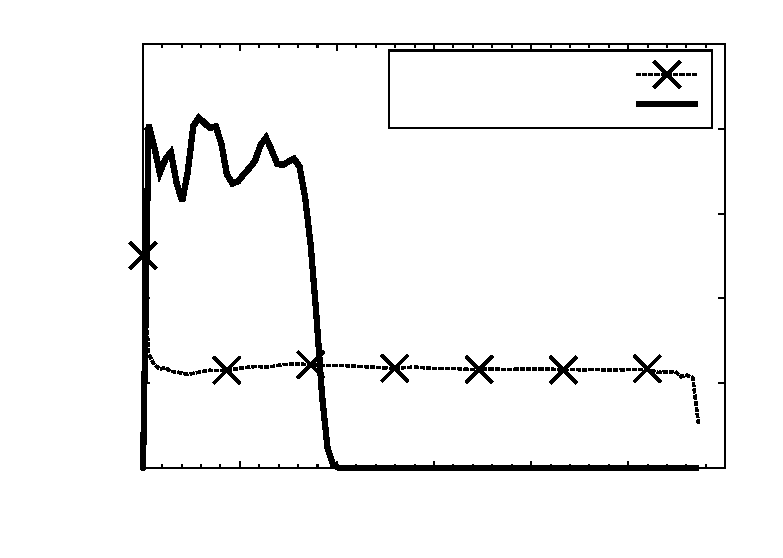
\includegraphics{graphs/replay/grafico_paper}}%
    \gplfronttext
  \end{picture}%
\endgroup
}
      }
      \subfloat[][Scalability \label{fig:scalability}]{
      \hspace{-0.7cm}
        \resizebox{4.5cm}{!}{% GNUPLOT: LaTeX picture with Postscript
\begingroup
  \makeatletter
  \providecommand\color[2][]{%
    \GenericError{(gnuplot) \space\space\space\@spaces}{%
      Package color not loaded in conjunction with
      terminal option `colourtext'%
    }{See the gnuplot documentation for explanation.%
    }{Either use 'blacktext' in gnuplot or load the package
      color.sty in LaTeX.}%
    \renewcommand\color[2][]{}%
  }%
  \providecommand\includegraphics[2][]{%
    \GenericError{(gnuplot) \space\space\space\@spaces}{%
      Package graphicx or graphics not loaded%
    }{See the gnuplot documentation for explanation.%
    }{The gnuplot epslatex terminal needs graphicx.sty or graphics.sty.}%
    \renewcommand\includegraphics[2][]{}%
  }%
  \providecommand\rotatebox[2]{#2}%
  \@ifundefined{ifGPcolor}{%
    \newif\ifGPcolor
    \GPcolorfalse
  }{}%
  \@ifundefined{ifGPblacktext}{%
    \newif\ifGPblacktext
    \GPblacktexttrue
  }{}%
  % define a \g@addto@macro without @ in the name:
  \let\gplgaddtomacro\g@addto@macro
  % define empty templates for all commands taking text:
  \gdef\gplbacktext{}%
  \gdef\gplfronttext{}%
  \makeatother
  \ifGPblacktext
    % no textcolor at all
    \def\colorrgb#1{}%
    \def\colorgray#1{}%
  \else
    % gray or color?
    \ifGPcolor
      \def\colorrgb#1{\color[rgb]{#1}}%
      \def\colorgray#1{\color[gray]{#1}}%
      \expandafter\def\csname LTw\endcsname{\color{white}}%
      \expandafter\def\csname LTb\endcsname{\color{black}}%
      \expandafter\def\csname LTa\endcsname{\color{black}}%
      \expandafter\def\csname LT0\endcsname{\color[rgb]{1,0,0}}%
      \expandafter\def\csname LT1\endcsname{\color[rgb]{0,1,0}}%
      \expandafter\def\csname LT2\endcsname{\color[rgb]{0,0,1}}%
      \expandafter\def\csname LT3\endcsname{\color[rgb]{1,0,1}}%
      \expandafter\def\csname LT4\endcsname{\color[rgb]{0,1,1}}%
      \expandafter\def\csname LT5\endcsname{\color[rgb]{1,1,0}}%
      \expandafter\def\csname LT6\endcsname{\color[rgb]{0,0,0}}%
      \expandafter\def\csname LT7\endcsname{\color[rgb]{1,0.3,0}}%
      \expandafter\def\csname LT8\endcsname{\color[rgb]{0.5,0.5,0.5}}%
    \else
      % gray
      \def\colorrgb#1{\color{black}}%
      \def\colorgray#1{\color[gray]{#1}}%
      \expandafter\def\csname LTw\endcsname{\color{white}}%
      \expandafter\def\csname LTb\endcsname{\color{black}}%
      \expandafter\def\csname LTa\endcsname{\color{black}}%
      \expandafter\def\csname LT0\endcsname{\color{black}}%
      \expandafter\def\csname LT1\endcsname{\color{black}}%
      \expandafter\def\csname LT2\endcsname{\color{black}}%
      \expandafter\def\csname LT3\endcsname{\color{black}}%
      \expandafter\def\csname LT4\endcsname{\color{black}}%
      \expandafter\def\csname LT5\endcsname{\color{black}}%
      \expandafter\def\csname LT6\endcsname{\color{black}}%
      \expandafter\def\csname LT7\endcsname{\color{black}}%
      \expandafter\def\csname LT8\endcsname{\color{black}}%
    \fi
  \fi
  \setlength{\unitlength}{0.0500bp}%
  \begin{picture}(7200.00,5040.00)%
    \gplgaddtomacro\gplbacktext{%
      \csname LTb\endcsname%
      \put(946,704){\makebox(0,0)[r]{\strut{} 0}}%
      \put(946,1156){\makebox(0,0)[r]{\strut{} 100}}%
      \put(946,1609){\makebox(0,0)[r]{\strut{} 200}}%
      \put(946,2061){\makebox(0,0)[r]{\strut{} 300}}%
      \put(946,2513){\makebox(0,0)[r]{\strut{} 400}}%
      \put(946,2966){\makebox(0,0)[r]{\strut{} 500}}%
      \put(946,3418){\makebox(0,0)[r]{\strut{} 600}}%
      \put(946,3870){\makebox(0,0)[r]{\strut{} 700}}%
      \put(946,4323){\makebox(0,0)[r]{\strut{} 800}}%
      \put(946,4775){\makebox(0,0)[r]{\strut{} 900}}%
      \put(1078,484){\makebox(0,0){\strut{} 0}}%
      \put(1896,484){\makebox(0,0){\strut{} 1}}%
      \put(2714,484){\makebox(0,0){\strut{} 2}}%
      \put(3532,484){\makebox(0,0){\strut{} 3}}%
      \put(4349,484){\makebox(0,0){\strut{} 4}}%
      \put(5167,484){\makebox(0,0){\strut{} 5}}%
      \put(5985,484){\makebox(0,0){\strut{} 6}}%
      \put(6803,484){\makebox(0,0){\strut{} 7}}%
      \put(176,2739){\rotatebox{-270}{\makebox(0,0){\strut{}Time to recovery (seconds)}}}%
      \put(3940,154){\makebox(0,0){\strut{}Number of application servers}}%
    }%
    \gplgaddtomacro\gplfronttext{%
      \csname LTb\endcsname%
      \put(5816,4481){\makebox(0,0)[r]{\strut{}1 replay; 1 database}}%
      \csname LTb\endcsname%
      \put(5816,4195){\makebox(0,0)[r]{\strut{}2 replay; 2 database}}%
    }%
    \gplbacktext
    \put(0,0){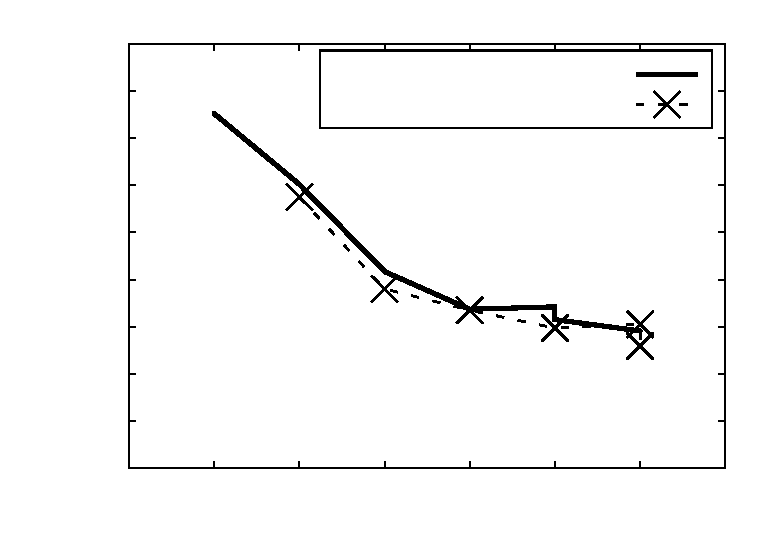
\includegraphics{graphs/scalability/recovery_time_paper}}%
    \gplfronttext
  \end{picture}%
\endgroup
}
      }
  }
  \caption{Recovery time and scalability}
  \vspace{-3mm}
\end{figure}

We measured the duration of the restrain period considering two clients with a constant throughput of 400 requests/sec. The serial replay mode, due to implementation issues, is not capable of exhausting the application servers and takes almost one hour to recover (2953s from which 1100s restraining) (Fig. \ref{fig:restrain:serial}). The clustered mode takes 10 minutes (635s), from which the restrain period represents 46 seconds. (Fig. \ref{fig:restrain:clustered}).

\begin{figure}[tbh]
\vspace{-5mm}
  \LARGE
  \mbox{
    \subfloat[][Serial \label{fig:restrain:serial}]{
      \hspace{-0.5cm}
      \resizebox{4.5cm}{!}{% GNUPLOT: LaTeX picture with Postscript
\begingroup
  \makeatletter
  \providecommand\color[2][]{%
    \GenericError{(gnuplot) \space\space\space\@spaces}{%
      Package color not loaded in conjunction with
      terminal option `colourtext'%
    }{See the gnuplot documentation for explanation.%
    }{Either use 'blacktext' in gnuplot or load the package
      color.sty in LaTeX.}%
    \renewcommand\color[2][]{}%
  }%
  \providecommand\includegraphics[2][]{%
    \GenericError{(gnuplot) \space\space\space\@spaces}{%
      Package graphicx or graphics not loaded%
    }{See the gnuplot documentation for explanation.%
    }{The gnuplot epslatex terminal needs graphicx.sty or graphics.sty.}%
    \renewcommand\includegraphics[2][]{}%
  }%
  \providecommand\rotatebox[2]{#2}%
  \@ifundefined{ifGPcolor}{%
    \newif\ifGPcolor
    \GPcolorfalse
  }{}%
  \@ifundefined{ifGPblacktext}{%
    \newif\ifGPblacktext
    \GPblacktexttrue
  }{}%
  % define a \g@addto@macro without @ in the name:
  \let\gplgaddtomacro\g@addto@macro
  % define empty templates for all commands taking text:
  \gdef\gplbacktext{}%
  \gdef\gplfronttext{}%
  \makeatother
  \ifGPblacktext
    % no textcolor at all
    \def\colorrgb#1{}%
    \def\colorgray#1{}%
  \else
    % gray or color?
    \ifGPcolor
      \def\colorrgb#1{\color[rgb]{#1}}%
      \def\colorgray#1{\color[gray]{#1}}%
      \expandafter\def\csname LTw\endcsname{\color{white}}%
      \expandafter\def\csname LTb\endcsname{\color{black}}%
      \expandafter\def\csname LTa\endcsname{\color{black}}%
      \expandafter\def\csname LT0\endcsname{\color[rgb]{1,0,0}}%
      \expandafter\def\csname LT1\endcsname{\color[rgb]{0,1,0}}%
      \expandafter\def\csname LT2\endcsname{\color[rgb]{0,0,1}}%
      \expandafter\def\csname LT3\endcsname{\color[rgb]{1,0,1}}%
      \expandafter\def\csname LT4\endcsname{\color[rgb]{0,1,1}}%
      \expandafter\def\csname LT5\endcsname{\color[rgb]{1,1,0}}%
      \expandafter\def\csname LT6\endcsname{\color[rgb]{0,0,0}}%
      \expandafter\def\csname LT7\endcsname{\color[rgb]{1,0.3,0}}%
      \expandafter\def\csname LT8\endcsname{\color[rgb]{0.5,0.5,0.5}}%
    \else
      % gray
      \def\colorrgb#1{\color{black}}%
      \def\colorgray#1{\color[gray]{#1}}%
      \expandafter\def\csname LTw\endcsname{\color{white}}%
      \expandafter\def\csname LTb\endcsname{\color{black}}%
      \expandafter\def\csname LTa\endcsname{\color{black}}%
      \expandafter\def\csname LT0\endcsname{\color{black}}%
      \expandafter\def\csname LT1\endcsname{\color{black}}%
      \expandafter\def\csname LT2\endcsname{\color{black}}%
      \expandafter\def\csname LT3\endcsname{\color{black}}%
      \expandafter\def\csname LT4\endcsname{\color{black}}%
      \expandafter\def\csname LT5\endcsname{\color{black}}%
      \expandafter\def\csname LT6\endcsname{\color{black}}%
      \expandafter\def\csname LT7\endcsname{\color{black}}%
      \expandafter\def\csname LT8\endcsname{\color{black}}%
    \fi
  \fi
  \setlength{\unitlength}{0.0500bp}%
  \begin{picture}(7200.00,5040.00)%
    \gplgaddtomacro\gplbacktext{%
      \csname LTb\endcsname%
      \put(1078,704){\makebox(0,0)[r]{\strut{} 0}}%
      \put(1078,1458){\makebox(0,0)[r]{\strut{} 500}}%
      \put(1078,2212){\makebox(0,0)[r]{\strut{} 1000}}%
      \put(1078,2966){\makebox(0,0)[r]{\strut{} 1500}}%
      \put(1078,3720){\makebox(0,0)[r]{\strut{} 2000}}%
      \put(1078,4473){\makebox(0,0)[r]{\strut{} 2500}}%
      \put(1210,484){\makebox(0,0){\strut{}00:00}}%
      \put(2329,484){\makebox(0,0){\strut{}10:00}}%
      \put(3447,484){\makebox(0,0){\strut{}20:00}}%
      \put(4566,484){\makebox(0,0){\strut{}30:00}}%
      \put(5684,484){\makebox(0,0){\strut{}40:00}}%
      \put(6803,484){\makebox(0,0){\strut{}50:00}}%
      \put(176,2739){\rotatebox{-270}{\makebox(0,0){\strut{}Requests per second}}}%
      \put(4006,154){\makebox(0,0){\strut{}Time (minutes:seconds)}}%
      \put(4659,2966){\makebox(0,0)[l]{\strut{}Restrain}}%
    }%
    \gplgaddtomacro\gplfronttext{%
      \csname LTb\endcsname%
      \put(2398,4481){\makebox(0,0)[r]{\strut{}serial}}%
      \csname LTb\endcsname%
      \put(2398,4195){\makebox(0,0)[r]{\strut{}client}}%
    }%
    \gplbacktext
    \put(0,0){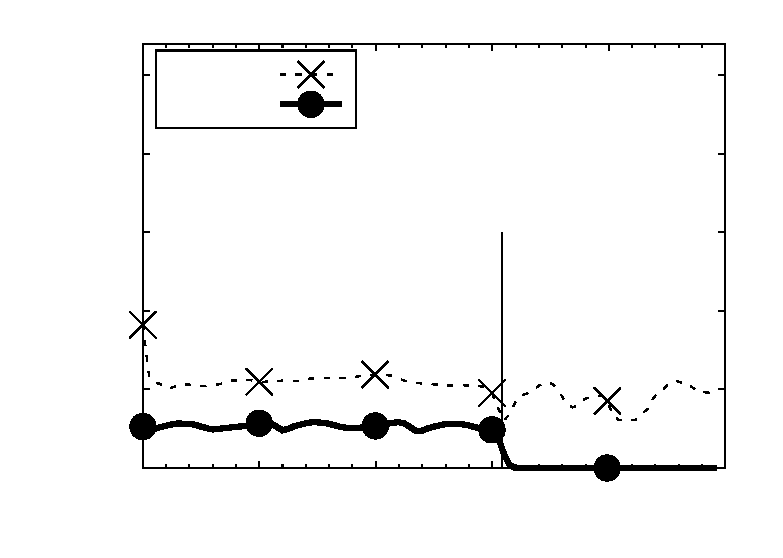
\includegraphics{graphs/restrain/serial_paper}}%
    \gplfronttext
  \end{picture}%
\endgroup
}
    }
    \subfloat[][Clustered \label{fig:restrain:clustered}]{
      \hspace{-0.7cm}
      \resizebox{4.5cm}{!}{% GNUPLOT: LaTeX picture with Postscript
\begingroup
  \makeatletter
  \providecommand\color[2][]{%
    \GenericError{(gnuplot) \space\space\space\@spaces}{%
      Package color not loaded in conjunction with
      terminal option `colourtext'%
    }{See the gnuplot documentation for explanation.%
    }{Either use 'blacktext' in gnuplot or load the package
      color.sty in LaTeX.}%
    \renewcommand\color[2][]{}%
  }%
  \providecommand\includegraphics[2][]{%
    \GenericError{(gnuplot) \space\space\space\@spaces}{%
      Package graphicx or graphics not loaded%
    }{See the gnuplot documentation for explanation.%
    }{The gnuplot epslatex terminal needs graphicx.sty or graphics.sty.}%
    \renewcommand\includegraphics[2][]{}%
  }%
  \providecommand\rotatebox[2]{#2}%
  \@ifundefined{ifGPcolor}{%
    \newif\ifGPcolor
    \GPcolorfalse
  }{}%
  \@ifundefined{ifGPblacktext}{%
    \newif\ifGPblacktext
    \GPblacktexttrue
  }{}%
  % define a \g@addto@macro without @ in the name:
  \let\gplgaddtomacro\g@addto@macro
  % define empty templates for all commands taking text:
  \gdef\gplbacktext{}%
  \gdef\gplfronttext{}%
  \makeatother
  \ifGPblacktext
    % no textcolor at all
    \def\colorrgb#1{}%
    \def\colorgray#1{}%
  \else
    % gray or color?
    \ifGPcolor
      \def\colorrgb#1{\color[rgb]{#1}}%
      \def\colorgray#1{\color[gray]{#1}}%
      \expandafter\def\csname LTw\endcsname{\color{white}}%
      \expandafter\def\csname LTb\endcsname{\color{black}}%
      \expandafter\def\csname LTa\endcsname{\color{black}}%
      \expandafter\def\csname LT0\endcsname{\color[rgb]{1,0,0}}%
      \expandafter\def\csname LT1\endcsname{\color[rgb]{0,1,0}}%
      \expandafter\def\csname LT2\endcsname{\color[rgb]{0,0,1}}%
      \expandafter\def\csname LT3\endcsname{\color[rgb]{1,0,1}}%
      \expandafter\def\csname LT4\endcsname{\color[rgb]{0,1,1}}%
      \expandafter\def\csname LT5\endcsname{\color[rgb]{1,1,0}}%
      \expandafter\def\csname LT6\endcsname{\color[rgb]{0,0,0}}%
      \expandafter\def\csname LT7\endcsname{\color[rgb]{1,0.3,0}}%
      \expandafter\def\csname LT8\endcsname{\color[rgb]{0.5,0.5,0.5}}%
    \else
      % gray
      \def\colorrgb#1{\color{black}}%
      \def\colorgray#1{\color[gray]{#1}}%
      \expandafter\def\csname LTw\endcsname{\color{white}}%
      \expandafter\def\csname LTb\endcsname{\color{black}}%
      \expandafter\def\csname LTa\endcsname{\color{black}}%
      \expandafter\def\csname LT0\endcsname{\color{black}}%
      \expandafter\def\csname LT1\endcsname{\color{black}}%
      \expandafter\def\csname LT2\endcsname{\color{black}}%
      \expandafter\def\csname LT3\endcsname{\color{black}}%
      \expandafter\def\csname LT4\endcsname{\color{black}}%
      \expandafter\def\csname LT5\endcsname{\color{black}}%
      \expandafter\def\csname LT6\endcsname{\color{black}}%
      \expandafter\def\csname LT7\endcsname{\color{black}}%
      \expandafter\def\csname LT8\endcsname{\color{black}}%
    \fi
  \fi
  \setlength{\unitlength}{0.0500bp}%
  \begin{picture}(7200.00,5040.00)%
    \gplgaddtomacro\gplbacktext{%
      \csname LTb\endcsname%
      \put(1078,704){\makebox(0,0)[r]{\strut{} 0}}%
      \put(1078,1458){\makebox(0,0)[r]{\strut{} 500}}%
      \put(1078,2212){\makebox(0,0)[r]{\strut{} 1000}}%
      \put(1078,2966){\makebox(0,0)[r]{\strut{} 1500}}%
      \put(1078,3720){\makebox(0,0)[r]{\strut{} 2000}}%
      \put(1078,4473){\makebox(0,0)[r]{\strut{} 2500}}%
      \put(1210,484){\makebox(0,0){\strut{}00:00}}%
      \put(2795,484){\makebox(0,0){\strut{}03:00}}%
      \put(4381,484){\makebox(0,0){\strut{}06:00}}%
      \put(5966,484){\makebox(0,0){\strut{}09:00}}%
      \put(176,2739){\rotatebox{-270}{\makebox(0,0){\strut{}Requests per second}}}%
      \put(4006,154){\makebox(0,0){\strut{}Time (minutes:seconds)}}%
      \put(5174,4473){\makebox(0,0)[l]{\strut{}Restrain}}%
    }%
    \gplgaddtomacro\gplfronttext{%
      \csname LTb\endcsname%
      \put(2794,4481){\makebox(0,0)[r]{\strut{}clustered}}%
      \csname LTb\endcsname%
      \put(2794,4195){\makebox(0,0)[r]{\strut{}client}}%
    }%
    \gplbacktext
    \put(0,0){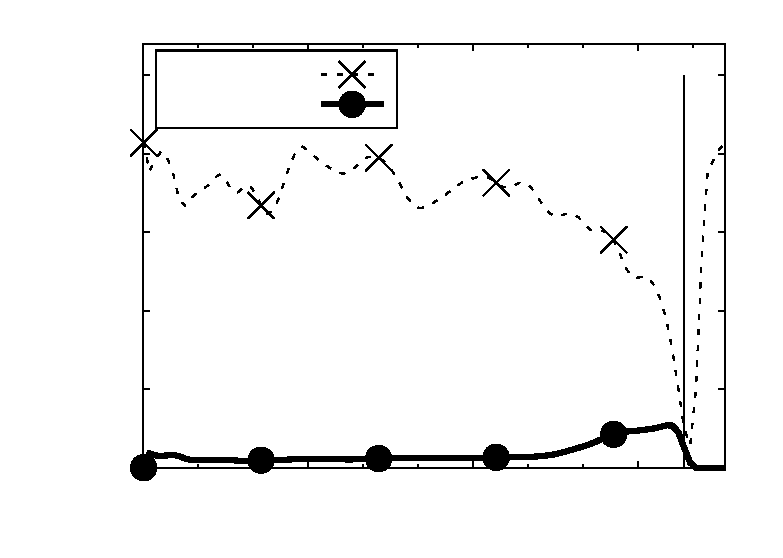
\includegraphics{graphs/restrain/clustered_paper}}%
    \gplfronttext
  \end{picture}%
\endgroup
}
    }
  }
  \caption{Restrain period in Serial and Parallel Recovery}
  \vspace{-3mm}
\end{figure}


\textbf{Space overhead.}
%Shuttle implies a fixed network overhead for attaching a \acf{SRD} (35 bytes) to every request and database access.
We measured the memory and storage overhead of 1 million requests, from which 95\% were read question requests. Values at Table \ref{tab:storage_overhead} represent the size of each component in memory \LONG{footnote{https://code.google.com/p/memory-measurer}}. Requests and keys are stored in the external database while the dependency graph and the accesses are kept in the manager and database instances. No snapshot has been taken and the data is not compressed.

In the current implementation, the \ac{SRD} represents a fixed overhead of 35 bytes per request.
\begin{table}[h]
\centering
\footnotesize
  \begin{tabular}{l|rr}
                & \# objects & size (MB) \\ \hline
  \textbf{Shuttle Storage: }      \\
  Request         & 1 million    & 212       \\  %1000000 - 212 162 883  old: & 200314    & 41,5 \\
  Response        & 1 million    & 8 967     \\  %1000000 - 8 967 233 474 old & 200314    & 1954 \\
  Start/End       & 2 million    & 16        \\  %2000000 - 16 000 000   old: & 200314    & 3,2  \\
  Keys            & 137 million  & 488       \\  %137 244 585  - 488 862 483 old: & 200314    & 105,2\\
  Total           &              & 9 684     \\  %9 684258 840
  \textbf{Database node:}        &           \\
  Version List    &  14 593      &  1.4       \\ %14 593 - 1 400 928   - 96 bytes old: & 3079     & 27,9 \\
  Operation list  &  9 million   &  277       \\ %9 551 908 - 277 019 984   - 29 bytes old: &  2061521  & 9,65 \\
  Total           &              & 282 \\ %282 230 960   old: & 61,3 \\
  \textbf{Manager:} & & \\ 
  Graph           & 1 million    & 718 \\  %718 486 432 old: & 200314    & 153,2 \\
  \end{tabular}            
\caption{Storage used by Shuttle}
\label{tab:storage_overhead}
\vspace{-5mm}
\end{table}

The main overhead are the responses, as we are storing them complete (the full HTML pages). Notice that Shuttle has to store the responses only if the tenant uses the API to solve inconsistencies (Section \ref{sec:recovery:consistency}). The size of the list of keys accessed by the request depends on the key length and the number of keys accessed. Each access implies an overhead of 13 bytes to record the request ID and the operation type in the version list. The snapshot does not impact the throughput but requires to track the new version, which implies a storage overhead of 10 bytes for each data item when it is written by the first time after a snapshot. The overhead can be reduced implementing the version list as a bitmap. The total database storage overhead encompasses synchronization mechanisms. Since the dependency graph is implemented as a double-linked graph, each entry in the dependency graph has 765 bytes to store not only the start/end instant of the request but also the requests which this request depends from and to (10 on average). Serialization mechanisms and compression techniques can reduce the storage overhead. For instance, the \emph{lz4} \LONG{cite{lz4}} of Cassandra, reduces th size of the Shuttle Storage in disk to 4.9 GB.

%For the sake of simplicity, the dependency graph is doubly-linked, a single-linked graph requires 458 bytes per entry. 
\textbf{Monetary cost.}
%\label{sec:evaluation:cost}
%
Since the replay instances are allocated on demand and paid-per usage, the cost of Shuttle is dominated by the storage. For instance, the proportional overhead of generating 20 million requests per day. To store a quarter (20 billion requests) requires 1.432 TB to store the Shuttle storage, 1.436 TB for the graph and 564 GB in the database instances. We propose to combine the DynamoDB to keep the last 24h of requests and the Glacier service to archive the data. Shuttle generates an average of 35 GB per day, which costs \$8.75 per month to store in DynamoDB and \$4.83 per-month for the provisioned capacity. The Glacier stores 3.433 TB so it costs \$34.33 per month. Since Shuttle performs snapshots, tenants can remove the old snapshots tacking into account that Shuttle needs only a snapshot previous to the intrusion instant to recover the application.

Shuttle requires an extra instance to deploy the Shuttle manager. To recover the application, we used one \emph{c3.xlarge} virtual machine as replay instance and two  \emph{c3.xlarge} instances to run the application servers to replay 1 million requests during 544 seconds. Considering a full-hour, these instances have an associated cost of \$0.239 per instance-hour, which means a cost of less than \$1 for the recovery. In this manner, Shuttle leverages the elasticity and pay-per-usage model of cloud computing to provide a cost-efficient intrusion recovery solution.